% ------------------------------------------------------------------------
% ------------------------------------------------------------------------
% abnTeX2: Modelo de Projeto de pesquisa em conformidade com 
% ABNT NBR 15287:2011 Informação e documentação - Projeto de pesquisa -
% Apresentação 
% ------------------------------------------------------------------------ 
% ------------------------------------------------------------------------

\documentclass[
% -- opções da classe memoir --
12pt,				% tamanho da fonte
openright,			% capítulos começam em pág ímpar (insere página vazia caso preciso)
oneside,			% para impressão em recto e verso. Oposto a oneside
a4paper,			% tamanho do papel. 
% -- opções da classe abntex2 --
chapter=TITLE,		% títulos de capítulos convertidos em letras maiúsculas
section=TITLE,		% títulos de seções convertidos em letras maiúsculas
%subsection=Title,	% títulos de subseções convertidos em letras maiúsculas
%subsubsection=TITLE,% títulos de subsubseções convertidos em letras maiúsculas
% -- opções do pacote babel --
english,			% idioma adicional para hifenização
brazil,				% o último idioma é o principal do documento
]{abntex2}

% ---
% PACOTES
% ---

% ---
% Pacotes fundamentais 
% ---
%\usepackage[latin1]{inputenc}
\usepackage[brazil]{babel}
\usepackage[T1]{fontenc}
\usepackage[utf8]{inputenc}		% Codificacao do documento
\usepackage{lmodern}			% Usa a fonte Latin Modern
\usepackage{indentfirst}		% Indenta o primeiro parágrafo de cada seção.
\usepackage{color}				% Controle das cores
\usepackage{graphicx}			% Inclusão de gráficos
\usepackage[export]{adjustbox}
\usepackage{microtype} 			% para melhorias de justificação
\usepackage{listings}
\usepackage{caption}
\usepackage{xcolor}
% ---


% ---
% Pacotes de citações
% ---
\usepackage[brazilian,hyperpageref]{backref}	 % Paginas com as citações na bibl
\usepackage[alf]{abntex2cite}	% Citações padrão ABNT
	% Incliu pacotes básicos 
% ---
% Configurações do pacote backref
% Usado sem a opção hyperpageref de backref
\renewcommand{\backrefpagesname}{Citado na(s) página(s):~}
% Texto padrão antes do número das páginas
\renewcommand{\backref}{}
% Define os textos da citação
\renewcommand*{\backrefalt}[4]{
	\ifcase #1 %
	Nenhuma citação no texto.%
	\or
	Citado na página #2.%
	\else
	Citado #1 vezes nas páginas #2.%
	\fi}%
% ---

% Ajusta os campos da capa
\renewcommand{\imprimircapa}{%
	\begin{capa}%
		\center
		{\normalsize\imprimirinstituicao}
		%{\ABNTEXchapterfont\normalsize\imprimirinstituicao}
		\vspace*{\fill}

		%{\ABNTEXchapterfont\normalsize\imprimirautor}
		{\normalsize\imprimirautor}
		
		\vspace*{\fill}
		%{\ABNTEXchapterfont\bfseries\normalsize\imprimirtitulo}
		{\normalsize\imprimirtitulo}
		
		\vspace*{\fill}
		{\normalsize\imprimirlocal}
		\par
		{\normalsize\imprimirdata}
		\vspace*{1cm}
		\end{capa}
}

% Ajusta os campos da contracapa

\makeatletter
\renewcommand{\folhaderostocontent}{
	\begin{center}
		{\normalsize\imprimirautor}
		
		
		\vspace*{\fill}\vspace*{\fill}
		{\normalsize\imprimirtitulo}
		\vspace*{\fill}
		
		\abntex@ifnotempty{\imprimirpreambulo}{%
			\hspace{.45\textwidth}
			\begin{minipage}{.5\textwidth}
				\SingleSpacing
				\imprimirpreambulo
			\end{minipage}%
			\vspace*{\fill}
		}%
		
		%{\abntex@ifnotempty{\imprimirinstituicao}{\imprimirinstituicao
		%		\vspace*{\fill}}}
		
		{\normalsize\imprimirorientadorRotulo~\imprimirorientador\par}
		\abntex@ifnotempty{\imprimircoorientador}{%
			{\normalsize\imprimircoorientadorRotulo~\imprimircoorientador}%
		}%
		\vspace*{\fill}
		
		{\normalsize\imprimirlocal}
		\par
		{\normalsize\imprimirdata}
		\vspace*{1cm}
		
	\end{center}
}
\makeatother

% Ajusta os contadores de seção para Modelo padrão do câmpus
\counterwithout{section}{section}
\counterwithout{figure}{chapter}
\counterwithout{table}{chapter}
\makepagestyle{plain}


% Ajusta o tamanho da fonte dos capítulos
\renewcommand{\ABNTEXchapterfontsize}{
	{\normalsize}
}	

% Ajusta o tamanho da fonte das seções
\renewcommand{\ABNTEXsectionfontsize}{
	{\normalsize}
}

% Ajusta o tamanho da fonte das subseções
\renewcommand{\ABNTEXsubsectionfontsize}{
	{\normalsize}
}		

% --- 
% Espaçamentos entre linhas e parágrafos 
% --- 

% O tamanho do parágrafo é dado por:
\setlength{\parindent}{1.3cm}

% Controle do espaçamento entre um parágrafo e outro:
\setlength{\parskip}{0.2cm}  % tente também \onelineskip

\definecolor{codegreen}{rgb}{0,0.6,0}
\definecolor{codegray}{rgb}{0.5,0.5,0.5}
\definecolor{codepurple}{rgb}{0.58,0,0.82}
\definecolor{backcolour}{rgb}{0.95,0.95,0.92}

\lstdefinestyle{mystyle}{
    backgroundcolor=\color{backcolour},   
    commentstyle=\color{codegreen},
    keywordstyle=\color{magenta},
    numberstyle=\tiny\color{codegray},
    stringstyle=\color{codepurple},
    basicstyle=\ttfamily\footnotesize,
    breakatwhitespace=false,         
    breaklines=true,                 
    captionpos=t,                    
    keepspaces=true,                 
    numbers=left,                    
    numbersep=5pt,                  
    showspaces=false,                
    showstringspaces=false,
    showtabs=false,                  
    tabsize=2
}

\lstset { %s
    style=mystyle,
    language=C++,
  	%basicstyle=\footnotesize,% basic font setting
  	%basicstyle=\ttfamily
}


\renewcommand{\lstlistingname}{Código}
% --- 
% SEUS AJUSTES DEVEM SER FEITOS ABAIXO DESSE COMENTÁRIO
% --- 
 % Inclui arquivo com reconfigurações.
% ---
% Informações de dados para CAPA e FOLHA DE ROSTO
% ---
\titulo{título aqui}
\autor{autor}
\orientador{Me. José Antônio Oliveira de Figueiredo}
%--\coorientador{nome}
\local{Passo Fundo}
\data{\the\year}
\instituicao{%
	INSTITUTO FEDERAL DE EDUCAÇÃO, CIÊNCIA E TECNOLOGIA 
	\par
	SUL-RIO-GRANDENSE - IFSUL, CÂMPUS PASSO FUNDO
	\par
	CURSO DE BACHARELADO EM CIÊNCIA DA COMPUTAÇÃO}
\tipotrabalho{Trabalho de conclusão de curso}
% O preambulo deve conter o tipo do trabalho, o objetivo, 
% o nome da instituição e a área de concentração 
\preambulo{Projeto de pesquisa submetido como requisito parcial para a aprovação na disciplina de Trabalho de Conclusão I do Curso de Ciência da Computação, do Instituto Federal Sul-Rio-Grandense, Câmpus Passo Fundo.}
% ---

% ---
% Configurações de aparência do PDF final

% alterando o aspecto da cor azul
\definecolor{blue}{RGB}{41,5,195}

% informações do PDF
\makeatletter
\hypersetup{
	%pagebackref=true,
	pdftitle={\@title}, 
	pdfauthor={\@author},
	pdfsubject={\imprimirpreambulo},
	pdfcreator={LaTeX with abnTeX2},
	pdfkeywords={keyword 1, keyword 2, keyword n}, 
	colorlinks=true,       		% false: boxed links; true: colored links
	linkcolor=blue,          	% color of internal links
	citecolor=blue,        		% color of links to bibliography
	filecolor=magenta,      		% color of file links
	urlcolor=blue,
	bookmarksdepth=4
}
\makeatother
% --- 


% ---
% compila o indice
% ---
\makeindex
% ---

% ----
% Início do documento
% ----
\begin{document}
	
	% Seleciona o idioma do documento (conforme pacotes do babel)
	%\selectlanguage{english}
	\selectlanguage{brazil}
	
	% Retira espaço extra obsoleto entre as frases.
	\frenchspacing 
	
	
	% ---
	% Capa
	% ---
	\imprimircapa
	% ---
	
	% ---
	% Folha de rosto
	% ---
	\imprimirfolhaderosto
	% ---
	
	
	% ---
	% inserir lista de ilustrações
	% ---
	%\pdfbookmark[0]{\listfigurename}{lof}
	%\listoffigures*
	%\cleardoublepage
	% ---
	
	% ---
	% inserir lista de tabelas
	% ---
	%\pdfbookmark[0]{\listtablename}{lot}
	%\listoftables*
	%\cleardoublepage
	% ---
	
	% ---
	% inserir lista de abreviaturas e siglas
	% ---
	%\begin{siglas}
	%	\item[ABNT] Associação Brasileira de Normas Técnicas
	%	\item[abnTeX] ABsurdas Normas para TeX
	%\end{siglas}
	% ---
	
	% ---
	% inserir lista de símbolos
	% ---
	%\begin{simbolos}
	%	\item[$ \Gamma $] Letra grega Gama
	%	\item[$ \Lambda $] Lambda
	%	\item[$ \zeta $] Letra grega minúscula zeta
	%	\item[$ \in $] Pertence
	%\end{simbolos}
	% ---
	
	% ---
	% inserir o sumario
	% ---
	\pdfbookmark[0]{\contentsname}{toc}
	\tableofcontents*
	\cleardoublepage
	% ---
	
	
% ----------------------------------------------------------
% ELEMENTOS TEXTUAIS
% ----------------------------------------------------------
\textual

%deixar chapter vazio - exatamente como está. Preencher o documento apenaas apartir de section.
\chapter*[]{}

\section{Tema}

texto aqui

\subsection{Delimitação do tema}

texto aqui

\section{Problema}

texto aqui


\section{Objetivos}
\subsection{Objetivo Geral}
texto aqui

\subsection{Objetivos Específicos}
\begin{enumerate}
\item texto aqui
\item texto aquiã.
\end{enumerate}

\section{Justificativa}

Segundo \citeonline{bourg2013physics}, texto aqui....

\citeonline{ericson2004real} texto aqui.

texto aqui
\section{Referencial Teórico}

texto aqui

\subsection{titulo de seção}

texto aqui 

texto aqui 

\subsubsection{titulo de sub seção}
texto aqui 

texto aqui

Exemplo de Quadro com Código - veja o quadro~\ref{code:vec_1}
\begin{lstlisting}[frame=single,caption=Exemplo de vetor 3d\label{code:vec_1}]
class vector3d{
  float x;
  float y;
  float z;

  vector3d(float x, float y, float z){
    this->x=x;
    this->y=y;
    this->z=z;
  }
};
\end{lstlisting}

\subsubsection{Caixas}

uma caixa é uma caixa... veja isso na Figura~\ref{fig:figura1}

\begin{figure}[htb]
  \centering
	\caption{\label{fig:figura1} Figura mostrando uma caixa}
	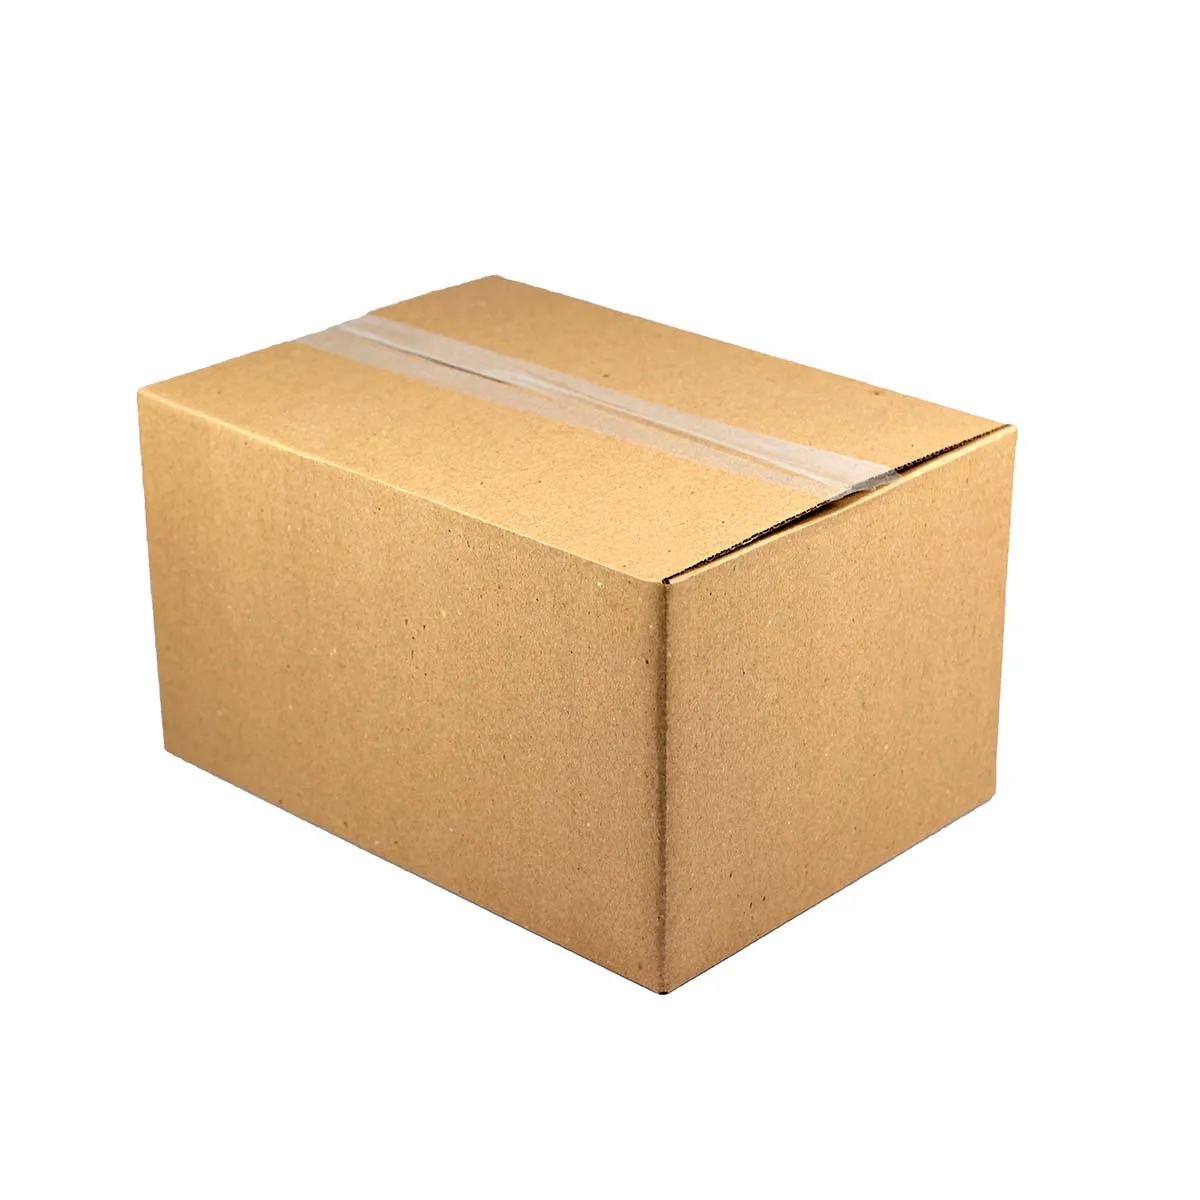
\includegraphics[scale=0.2]{Imagens/figura1.png} %width=\textwidth
	\legend{Fonte: \cite{ericson2004real}. }
\end{figure}




\section{Metodologia}

texto aqui 

\subsection{sub seção }

texto aqui 


\subsection{Recursos necessários}

Lista dos Recursos 

\begin{itemize}
\item item 1;
\item item 2;
\end{itemize}

\subsection{Cronograma}

A listagem a seguir, apresenta uma distribuição estimada das tarefas a serem
realizadas de forma quinzenal.

aqui vai o cronograma em forma de tabela.



% ---
% Finaliza a parte no bookmark do PDF
% para que se inicie o bookmark na raiz
% e adiciona espaço de parte no Sumário
% ---
\phantompart

% ----------------------------------------------------------
% ELEMENTOS PÓS-TEXTUAIS
% ----------------------------------------------------------
\postextual

% ----------------------------------------------------------
% Referências bibliográficas
% ----------------------------------------------------------
\bibliography{bibliografia}


\end{document}
